% Look!  A mock introduction

% The introduction is one of the most important pieces of your thesis.  Here is a place for you to introduce the problem(s) on which you have worked and place them in the larger context of your field.  You should aim to ensure that this section is completely understandable to virtually anyone - and certainly anyone with a sophomore-level grasp of physics.  Presumably this will include references to the literature.

% In addition to setting your work into context, a second good idea for your introduction is to give a short outline for what the rest of your thesis will discuss.  This is often done in the closing paragraph(s) of the introduction with sentences like ``In the following chapters \ldots " and ``Chapter 2 discusses \ldots"  Tremendous detail is not required in this outline, but rather just a brief road map for the rest of the document.

This thesis centers on the modeling of Passive Daytime Radiative Cooling Devices (PDRCs) utilizing the COMSOL Multiphysics™ software. While all objects with a temperature above absolute zero emit blackbody radiation, PDRCs are distinct in their ability to efficiently radiate heat in the mid-infrared range where the Earth's atmosphere is most transparent. This allows PDRCs to effectively transfer heat directly to the cold sink of outer space during daylight hours, without the need for electrical energy. Therefore, PDRCs hold the promise of addressing two significant challenges: the energy crisis and global warming. % rephrased

\section{Cooling is Critical}
Over the years, cooling has become more critical to humans due to global warming, rapid population growth and industrial development \cite{chen_passive_2022}. Various methods exist for cooling buildings, ranging from traditional practices, such as shading and solar orientation, to the use of electric fans. The most advanced approach is air conditioning (AC), encompassing systems that enhance indoor thermal comfort and air quality. While mechanical cooling techniques date back to the 19th century, widespread adoption of air conditioning began in the 1950s, driven by improved performance, affordability, and economic prosperity, primarily in the United States \cite{international_energy_agency_future_2018}.

Modern AC systems vary widely in size and cost, catering to individual rooms or entire buildings, with electricity being the predominant power source. Today, the largest concentration of cooling systems is found in urban areas, both in industrialized nations and emerging economies, reflecting the higher population density and greater demand for climate control in these regions \cite{international_energy_agency_future_2018}. 

Particularly in the realm of residential air conditioners (ACs), China emerges as the foremost market with a staggering sale of 41 million units. Following China, Japan and the European Union represent the subsequent largest markets for residential ACs. However, there is a significant uptick in sales within various emerging economies, notably in Asia (see figure \ref{fig:sales_acs}).

Global sales of ACs have exhibited consistent growth in recent years. Over the period from 1990 to 2016, annual AC sales experienced a nearly fourfold increase, reaching 135 million units. In 2016, China emerged as the leading market in terms of AC capacity sales, totaling nearly 390 gigawatts (53 million units) \cite{international_energy_agency_future_2018}. % rephrased

\begin{figure}
  \centering
  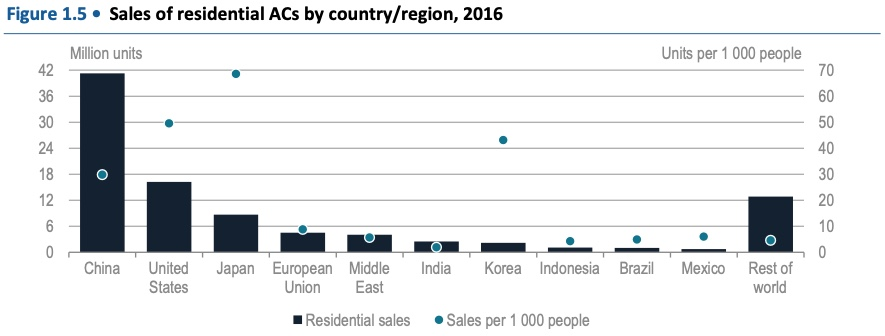
\includegraphics[width=0.8\textwidth]{Chapters/Figures/Sales of Residential ACs by Country or Region, 2016.jpg}
  \caption[Sales of Residential ACs by Country or Region, 2016]{Sales of Residential ACs by Country or Region, 2016. Source: \cite{international_energy_agency_future_2018}.}
  \label{fig:sales_acs}
\end{figure}

The growing demand for cooling is significantly influencing power systems, primarily due to the reliance on electricity-driven fans or air conditioners to meet cooling requirements. The escalating demand for air conditioning, in particular, not only elevates overall electricity consumption but also contributes to higher peak electricity loads. Additionally, the emission of greenhouse gases (GHGs) from ACs occurs through refrigerant leakage or improper disposal. It's noteworthy that these refrigerants are potent GHGs with adverse implications for climate change \cite{international_energy_agency_future_2018}. % (INTERNATIONAL ENERGY AGENCY, 2018) % rephrased

Improving the efficiency of air conditioning systems (ACs) is pivotal in mitigating peak electricity demand, thereby resulting in decreased emissions and associated financial implications. Endeavors focused on enhancing cooling efficiency necessitate a thorough assessment of the comparative costs linked to diverse cooling technologies. % rephrased

\section{Radiative Cooling}

\begin{figure}
  \centering
  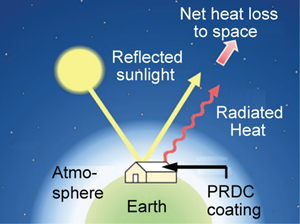
\includegraphics[width=0.4\textwidth]{Chapters/Figures/Schematic for Radiative Cooling.png}
  \caption[Schematic for Radiative Cooling] {Schematic for Radiative Cooling. Source: \cite{yang_passive_2020}}
  \label{fig:PDRC_Schematic}
\end{figure}

Objects with temperatures above absolute zero emit blackbody radiation, with a spectrum that depends on their temperature as governed by Planck's law. While the emitted radiation covers a range of wavelengths, it is not uniformly distributed across all wavelengths. Radiative passive cooling occurs when objects emit more radiation, particularly in the infrared spectrum, than the combined radiation they absorb, which includes both blackbody and solar radiation. Thus radiative passive cooling is an electricity-free method for cooling terrestrial entities \cite{yang_passive_2020}.

The heat emitted by these objects, which exceeds the heat they absorb, is transferred to outer space via thermal radiation, leveraging the substantial temperature difference between Earth (approximately 300 K) and outer space (approximately 3 K) (See figure \ref{fig:PDRC_Schematic} for net heat loss to space). This process efficiently exchanges heat with the infinite cold reservoir of deep space, achieving cooling without any energy consumption \cite{chen_passive_2022}.

Passive radiative cooling can be realized even during the daytime, necessitating precise tuning of optical properties across a broad spectrum of wavelengths, from ultraviolet to mid-infrared (see figure \ref{fig:ideal_PDRC_properties}). As a result, achieving effective passive daytime radiative cooling imposes stringent requirements on materials and structures to mitigate solar heating \cite{yang_passive_2020}:

\begin{enumerate} 
\item Minimal absorptivity ($\alpha$) approaching 0\% (equivalent to nearly 100\% reflectance, $R$) in the solar spectrum, ranging from 0.3–2.5 $\mu m$. This characteristic ensures that the surface absorbs minimal solar energy during daylight, thereby reducing the heat gained by the PDRC.
\item High thermal radiation in the atmospheric transparency window, with an emittance ($\varepsilon$) close to 1 within the long-wavelength infrared (LWIR) transmission window of the atmosphere ($\lambda$ = 8–13 $\mu m$). This range is significant due to the atmosphere's partial transparency and minimal infrared absorption by gas molecules in this spectrum.
\item An emittance ($\varepsilon$) close to 0 in other mid-infrared wavelengths, such as 5–8 $\mu m$ and those greater than 13 $\mu m$. This characteristic is crucial due to the atmosphere's opacity in these spectral ranges.
\end{enumerate}

% NB: Using [ht!] tells LaTeX to try to place the figure here, but if that's not possible, then at the top of the page, and the ! overrides LaTeX's internal parameters for deciding on figure placements. This gives you the best chance of having the figure appear right after your enumerated list, although it's not a guarantee because LaTeX might still decide to move the figure based on its page layout algorithms.
\begin{figure}[ht!]
  \centering
  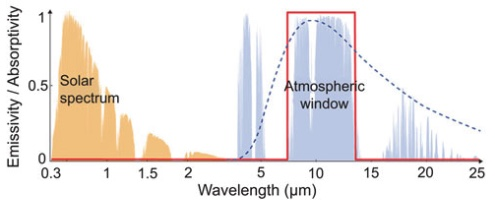
\includegraphics[width=0.4\textwidth]{Chapters/Figures/Ideal Optical Properties of a Radiative Cooling Surface.jpg}
  \caption[Ideal Optical Properties of a Radiative Cooling Surface]{Ideal Optical Properties of a Radiative Cooling Surface. Source: \cite{yang_passive_2020}}
  \label{fig:ideal_PDRC_properties}
\end{figure}


% -- SECTION 1.3: LITERATURE REVIEW ---

\section{Literature Review}
At the nexus of physics and technological advancement, Passive Daytime Radiative Cooling Devices (PDRCs) stand as a symbol of optimism amidst the challenges of global warming and the energy crisis. PDRCs are notable not just for their operational efficiency but also for their capacity to transform our approach to energy consumption and environmental conservation.

While radiative cooling for nighttime use was established decades ago, only recently has there been significant progress in achieving cooling directly under sunlight, suggesting a promising upward trajectory for the technology's cooling capabilities.

In 1965, French Engineer Félix Trombe introduced the concept of Radiative Cooling. Collaborating with A. Le Phat Vinh and Mrs. M. Le Phat Vinh at Montlouis Laboratory, they explored radiative cooling to achieve significantly larger temperature reductions than naturally occur. They developed a method to dissipate heat into the sky without insulation, using a system that could lower temperatures by 14 to 30 degrees Celsius compared to the environment. This system involved a north-facing, slightly tilted facade with infrared-transparent panels and a selective radiator, optimizing both night and daytime cooling. % TROMBE % FORTIN

\emph{Following Trombe's pioneering work, Catalanotti and colleagues in 1975 crafted an experimental setup for daytime radiative cooling using a combination of metals and TEDLAR (polyvinyl-fluoride plastic), designed to shield the radiator from direct sunlight, yet it primarily enhanced nighttime cooling. [5]. Subsequent attempts included using thin films coated on aluminum substrates with specific material compositions, such as coated thin solid film on an aluminum substrate with $\text{SiO}_6\text{N}_{0.2}$ [6] and double layers of $\text{SiO}_2$ and $\text{SiO}_{0.25}\text{N}_{1.52}$, to achieve selective spectral emission. However, these efforts faced challenges in realizing effective daytime radiative cooling.}
% BIJARNIYA % [5]=The radiative cooling of selective surfaces % [6]=Materials for radiative cooling to low temperature % [7]=Surface coatings for radiative cooling applications: Silicon dioxide and silicon nitride made by reactive rf-sputtering

Continuous efforts have been made to increase the cooling efficiency of radiative emitters and as evidenced above, practical cooling at night was also demonstrated. However, the use of naturally available materials and synthetic polymers has always been the limiting factor. The lack of suitable materials with high solar reflection but possessing strong emission within the IR window restricted any effective radiative cooling under the direct sunlight. % HOSSAIN AND GU

Selective IR emitters of various bulk materials have been studied and among them are polymer films, white pigmented paints, silicon monoxide (SiO) films and others. However, one major disadvantage is that many of them suffer from weak emissivity, limiting the cooling performance. Moreover, the lack of strict selectivity of the IR emission/absorption, results in significant absorption of the atmospheric radiation outside the transparency window, not allowing the cooling device to achieve steady state temperature significantly below the ambient temperature. % HOSSAIN AND GU

Catalanotti and colleagues and Bartoli and collegues utilized a commercially avail- able polyvinyl-fluoride polymer film (TEDLAR) as the radiative emitter which possesses somewhat selective and high IR absorption from 9 to 13 $\mu m$ wavelengths range. However, significant IR absorption also occurs beyond 20 $\mu m$. This weak selectivity limits the radiative cooling efficiency of the polymer film. Catalanotti and Bartoli demonstrated a temperature reduction of 10 degrees Celsius below the ambient during the daytime but only under diffused sunlight conditions. The main limitation, however, of polyvinyl-fluoride (PVF) polymer they used for radiative cooling during the day is due to its significant optical absorption within the solar spectra.

Other types of polymer films, polyvinylchloride (PVC) and poly(4- methylpentene) (TPX) have also been investigated for radiative cooling but their IR emissivity profiles are worse than those of PVF in terms of selectivity and strong emission within the vital 8-13 $\mu m$ range.

Pigmented paints, naturally available inorganic compounds and gases with IR emission were also investigated for nocturnal radiative cooling applications. Commercially available white paint containing titanium dioxide (TiO$_2$) was coated on aluminum plates and was used as the IR radiator. Although realistic cooling was not achieved directly under the sun at mid noon, a steady cooling of around 10 °C below the ambient temperature under clear sky conditions was reported during the night. On a relatively low humid day a maximum cooling 15 °C below the ambient was also demonstrated. Pigmented paints thus may have advantages over polymer films for nocturnal radiative cooling applications due to the flexibility of coating any suitable substrates with easily available regular paints.

The utilization of Silicon Dioxide (SiO) films and other inorganic materials for infrared (IR) emission in the context of radiative cooling devices focuses on their ability to emit thermal radiation within specific wavelengths. These materials have been explored for their potential to enhance cooling by radiating heat away from surfaces. However, one limitation is their narrow emission bandwidth, which can restrict the overall effectiveness of cooling. A narrow bandwidth means that the range of wavelengths over which these materials can emit IR radiation efficiently is limited, potentially reducing the amount of heat that can be dissipated into the atmosphere and ultimately impacting the cooling performance of the device.

The exploration of solar reflectors and IR-transparent materials for daytime radiative cooling has shown promise in reflecting solar radiation and enabling infrared (IR) emission. This dual functionality is critical for cooling during daylight by preventing solar heat gain while facilitating the emission of thermal energy from the surface. However, achieving effective cooling during peak sunlight hours poses a significant challenge due to the intense solar irradiance. The balance between reflecting enough solar radiation to prevent heating and allowing sufficient IR emission for cooling is difficult to achieve, especially under direct sunlight conditions.

Apart from solar reflectors, convection covers can also play important role to optimize the performance of the radiative cooler. For daytime applications, if the cooling device’s net radiated power (i.e., $P_r - P_a$) is higher than the absorbed solar power (i.e., for a cooler with high solar reflectance), the device can yield a temperature well below the ambient temperature provided that convective heat gain is suppressed. In this circumstance, the use of convective covers is undesirable as natural convection can aid to release heat from the cooling device. In the absence of direct solar radiation convection covers can greatly improve the performances for maximum cooling.

Recent progress on developing radiative coolers based on photonic devices has opened a new window to achieve highly efficient cooling and the ability to operate directly under the sun, reaching temperature below the ambient temperature. Unlike radiative coolers based on the intrinsic optical properties of bulk materials, these approaches utilize engineered photonic properties combined with the intrinsic properties to realize improved cooling abilities.

The first experimental demonstration of radiative cooling with planar photonic devices operating directly under the sun was reported by Raman et al. where, a temperature reduction of 4.9 degrees Celsius below the ambient temperature was achieved. The photonic device consisted of seven alternating layers of hafnium oxide (HfO2) and SiO2 with varying thickness. The top three thick layers mainly contributed to the IR emissivity including the 8–13 $\mu m$ wavelengths range and the four thinner bottom layers deposited on Al coated Si wafer worked as chirped 1D photonic crystal for a maximum of 97\% solar reflection.

The challenge for this device for achieving further cooling lies between the IR emission properties of HfO2 and SiO2. First, the IR emission of the device is not strictly selective, which is due to the broadband intrinsic absorption of the mate- rials. Second, the emission within the 8–13 $\mu m$ wavelengths range is not very strong. Increasing the thickness of the top three layers may increase the IR emission; however, may also degrade the selectivity of the IR emission. The choice of using the same materials for IR emission and solar restriction has also restricted the flexibility to further optimize the device for improved cooling power.

% TODO: Attach figure 5 (a) in the Hossaini and Gu paper.


% B. BARTOLI, S. Catalanotti, B. Coluzzi, V. Cuomo, V. Silvestrini, G. Troise, Appl. Energy 1977, 3, 267.


% -- SECTION 1.4: PREVIOUS PROJECT WORK AND PROJECT GOALS ---

\section{Previous Project Work and Project Goals}
Research on PDRCs has been an ongoing project in the Hudgings lab. This thesis aims to build upon the work of Paul McKinley (class of 2022) and Genevieve diBari (class of 2023).

McKinley laid the groundwork by developing a rooftop testbed and the fabrication process for PDRCs (a process I plan to replicate after completing the modeling of various PDRC iterations on COMSOL). DiBari contributed by modeling PDRCs in Python and enhancing the initial outdoor testing setup.

For my thesis, the goal is to model different PDRC structures using COMSOL, exploring materials that could enhance the optical properties of an ideal PDRC device. This includes stacking materials of varying thicknesses and refractive indices on current PDRC models in the Hudgings lab to increase reflectivity ($R$). If time permits, promising PDRC models (with high $R$ and/or emissivity in the atmospheric window) will be fabricated after the modeling phase.
